\documentclass[1p]{elsarticle_modified}
%\bibliographystyle{elsarticle-num}

%\usepackage[colorlinks]{hyperref}
%\usepackage{abbrmath_seonhwa} %\Abb, \Ascr, \Acal ,\Abf, \Afrak
\usepackage{amsfonts}
\usepackage{amssymb}
\usepackage{amsmath}
\usepackage{amsthm}
\usepackage{scalefnt}
\usepackage{amsbsy}
\usepackage{kotex}
\usepackage{caption}
\usepackage{subfig}
\usepackage{color}
\usepackage{graphicx}
\usepackage{xcolor} %% white, black, red, green, blue, cyan, magenta, yellow
\usepackage{float}
\usepackage{setspace}
\usepackage{hyperref}

\usepackage{tikz}
\usetikzlibrary{arrows}

\usepackage{multirow}
\usepackage{array} % fixed length table
\usepackage{hhline}

%%%%%%%%%%%%%%%%%%%%%
\makeatletter
\renewcommand*\env@matrix[1][\arraystretch]{%
	\edef\arraystretch{#1}%
	\hskip -\arraycolsep
	\let\@ifnextchar\new@ifnextchar
	\array{*\c@MaxMatrixCols c}}
\makeatother %https://tex.stackexchange.com/questions/14071/how-can-i-increase-the-line-spacing-in-a-matrix
%%%%%%%%%%%%%%%

\usepackage[normalem]{ulem}

\newcommand{\msout}[1]{\ifmmode\text{\sout{\ensuremath{#1}}}\else\sout{#1}\fi}
%SOURCE: \msout is \stkout macro in https://tex.stackexchange.com/questions/20609/strikeout-in-math-mode

\newcommand{\cancel}[1]{
	\ifmmode
	{\color{red}\msout{#1}}
	\else
	{\color{red}\sout{#1}}
	\fi
}

\newcommand{\add}[1]{
	{\color{blue}\uwave{#1}}
}

\newcommand{\replace}[2]{
	\ifmmode
	{\color{red}\msout{#1}}{\color{blue}\uwave{#2}}
	\else
	{\color{red}\sout{#1}}{\color{blue}\uwave{#2}}
	\fi
}

\newcommand{\Sol}{\mathcal{S}} %segment
\newcommand{\D}{D} %diagram
\newcommand{\A}{\mathcal{A}} %arc


%%%%%%%%%%%%%%%%%%%%%%%%%%%%%5 test

\def\sl{\operatorname{\textup{SL}}(2,\Cbb)}
\def\psl{\operatorname{\textup{PSL}}(2,\Cbb)}
\def\quan{\mkern 1mu \triangleright \mkern 1mu}

\theoremstyle{definition}
\newtheorem{thm}{Theorem}[section]
\newtheorem{prop}[thm]{Proposition}
\newtheorem{lem}[thm]{Lemma}
\newtheorem{ques}[thm]{Question}
\newtheorem{cor}[thm]{Corollary}
\newtheorem{defn}[thm]{Definition}
\newtheorem{exam}[thm]{Example}
\newtheorem{rmk}[thm]{Remark}
\newtheorem{alg}[thm]{Algorithm}

\newcommand{\I}{\sqrt{-1}}
\begin{document}

%\begin{frontmatter}
%
%\title{Boundary parabolic representations of knots up to 8 crossings}
%
%%% Group authors per affiliation:
%\author{Yunhi Cho} 
%\address{Department of Mathematics, University of Seoul, Seoul, Korea}
%\ead{yhcho@uos.ac.kr}
%
%
%\author{Seonhwa Kim} %\fnref{s_kim}}
%\address{Center for Geometry and Physics, Institute for Basic Science, Pohang, 37673, Korea}
%\ead{ryeona17@ibs.re.kr}
%
%\author{Hyuk Kim}
%\address{Department of Mathematical Sciences, Seoul National University, Seoul 08826, Korea}
%\ead{hyukkim@snu.ac.kr}
%
%\author{Seokbeom Yoon}
%\address{Department of Mathematical Sciences, Seoul National University, Seoul, 08826,  Korea}
%\ead{sbyoon15@snu.ac.kr}
%
%\begin{abstract}
%We find all boundary parabolic representation of knots up to 8 crossings.
%
%\end{abstract}
%\begin{keyword}
%    \MSC[2010] 57M25 
%\end{keyword}
%
%\end{frontmatter}

%\linenumbers
%\tableofcontents
%
\newcommand\colored[1]{\textcolor{white}{\rule[-0.35ex]{0.8em}{1.4ex}}\kern-0.8em\color{red} #1}%
%\newcommand\colored[1]{\textcolor{white}{ #1}\kern-2.17ex	\textcolor{white}{ #1}\kern-1.81ex	\textcolor{white}{ #1}\kern-2.15ex\color{red}#1	}

{\Large $\underline{12n_{0397}~(K12n_{0397})}$}

\setlength{\tabcolsep}{10pt}
\renewcommand{\arraystretch}{1.6}
\vspace{1cm}\begin{tabular}{m{100pt}>{\centering\arraybackslash}m{274pt}}
\multirow{5}{120pt}{
	\centering
	\includegraphics[width=112pt]{../../../GIT/diagram.site/Diagrams/png/2486_12n_0397.png}\\
\ \ \ A knot diagram\footnotemark}&
\allowdisplaybreaks
\textbf{Linearized knot diagam} \\
\cline{2-2}
 &
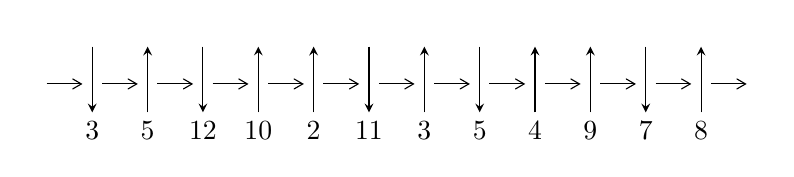
\begin{tikzpicture}[x=20pt, y=17pt]
	% nodes
	\node (C0) at (0, 0) {};
	\node (C1) at (1, 0) {};
	\node (C1U) at (1, +1) {};
	\node (C1D) at (1, -1) {3};

	\node (C2) at (2, 0) {};
	\node (C2U) at (2, +1) {};
	\node (C2D) at (2, -1) {5};

	\node (C3) at (3, 0) {};
	\node (C3U) at (3, +1) {};
	\node (C3D) at (3, -1) {12};

	\node (C4) at (4, 0) {};
	\node (C4U) at (4, +1) {};
	\node (C4D) at (4, -1) {10};

	\node (C5) at (5, 0) {};
	\node (C5U) at (5, +1) {};
	\node (C5D) at (5, -1) {2};

	\node (C6) at (6, 0) {};
	\node (C6U) at (6, +1) {};
	\node (C6D) at (6, -1) {11};

	\node (C7) at (7, 0) {};
	\node (C7U) at (7, +1) {};
	\node (C7D) at (7, -1) {3};

	\node (C8) at (8, 0) {};
	\node (C8U) at (8, +1) {};
	\node (C8D) at (8, -1) {5};

	\node (C9) at (9, 0) {};
	\node (C9U) at (9, +1) {};
	\node (C9D) at (9, -1) {4};

	\node (C10) at (10, 0) {};
	\node (C10U) at (10, +1) {};
	\node (C10D) at (10, -1) {9};

	\node (C11) at (11, 0) {};
	\node (C11U) at (11, +1) {};
	\node (C11D) at (11, -1) {7};

	\node (C12) at (12, 0) {};
	\node (C12U) at (12, +1) {};
	\node (C12D) at (12, -1) {8};
	\node (C13) at (13, 0) {};

	% arrows
	\draw[->,>={angle 60}]
	(C0) edge (C1) (C1) edge (C2) (C2) edge (C3) (C3) edge (C4) (C4) edge (C5) (C5) edge (C6) (C6) edge (C7) (C7) edge (C8) (C8) edge (C9) (C9) edge (C10) (C10) edge (C11) (C11) edge (C12) (C12) edge (C13) ;	\draw[->,>=stealth]
	(C1U) edge (C1D) (C2D) edge (C2U) (C3U) edge (C3D) (C4D) edge (C4U) (C5D) edge (C5U) (C6U) edge (C6D) (C7D) edge (C7U) (C8U) edge (C8D) (C9D) edge (C9U) (C10D) edge (C10U) (C11U) edge (C11D) (C12D) edge (C12U) ;
	\end{tikzpicture} \\
\hhline{~~} \\& 
\textbf{Solving Sequence} \\ \cline{2-2} 
 &
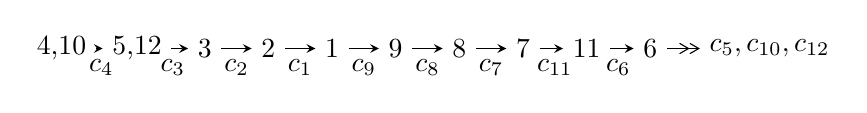
\begin{tikzpicture}[x=23pt, y=7pt]
	% node
	\node (A0) at (-1/8, 0) {4,10};
	\node (A1) at (17/16, 0) {5,12};
	\node (A2) at (17/8, 0) {3};
	\node (A3) at (25/8, 0) {2};
	\node (A4) at (33/8, 0) {1};
	\node (A5) at (41/8, 0) {9};
	\node (A6) at (49/8, 0) {8};
	\node (A7) at (57/8, 0) {7};
	\node (A8) at (65/8, 0) {11};
	\node (A9) at (73/8, 0) {6};
	\node (C1) at (1/2, -1) {$c_{4}$};
	\node (C2) at (13/8, -1) {$c_{3}$};
	\node (C3) at (21/8, -1) {$c_{2}$};
	\node (C4) at (29/8, -1) {$c_{1}$};
	\node (C5) at (37/8, -1) {$c_{9}$};
	\node (C6) at (45/8, -1) {$c_{8}$};
	\node (C7) at (53/8, -1) {$c_{7}$};
	\node (C8) at (61/8, -1) {$c_{11}$};
	\node (C9) at (69/8, -1) {$c_{6}$};
	\node (A10) at (11, 0) {$c_{5},c_{10},c_{12}$};

	% edge
	\draw[->,>=stealth]	
	(A0) edge (A1) (A1) edge (A2) (A2) edge (A3) (A3) edge (A4) (A4) edge (A5) (A5) edge (A6) (A6) edge (A7) (A7) edge (A8) (A8) edge (A9) ;
	\draw[->>,>={angle 60}]	
	(A9) edge (A10);
\end{tikzpicture} \\ 

\end{tabular} \\

\footnotetext{
The image of knot diagram is generated by the software ``\textbf{Draw programme}" developed by Andrew Bartholomew(\url{http://www.layer8.co.uk/maths/draw/index.htm\#Running-draw}), where we modified some parts for our purpose(\url{https://github.com/CATsTAILs/LinksPainter}).
}\phantom \\ \newline 
\centering \textbf{Ideals for irreducible components\footnotemark of $X_{\text{par}}$} 
 
\begin{align*}
I^u_{1}&=\langle 
u^{23}+8 u^{22}+\cdots+2 b+26,\;-23 u^{23}-133 u^{22}+\cdots+8 a-112,\;u^{24}+7 u^{23}+\cdots+44 u+8\rangle \\
I^u_{2}&=\langle 
2 u^{17}-9 u^{15}+21 u^{13}-28 u^{11}+2 u^{10}+23 u^9-7 u^8-7 u^7+10 u^6-5 u^5-6 u^4+7 u^3+b-3 u+1,\\
\phantom{I^u_{2}}&\phantom{= \langle  }-2 u^{17}+u^{16}+\cdots+a-3,\\
\phantom{I^u_{2}}&\phantom{= \langle  }u^{18}-5 u^{16}+13 u^{14}-20 u^{12}+u^{11}+20 u^{10}-4 u^9-11 u^8+7 u^7+u^6-6 u^5+4 u^4+2 u^3-3 u^2+1\rangle \\
I^u_{3}&=\langle 
109 a^3 u^2-389 a^2 u^2+\cdots+1134 a-188,\;a^4+a^3 u+a^2 u^2- a^3-10 a^2 u-5 u^2 a-3 a u-5 a-4 u-1,\\
\phantom{I^u_{3}}&\phantom{= \langle  }u^3- u^2+1\rangle \\
I^u_{4}&=\langle 
b+u,\;a^2+a u+4 u^2-6 u+4,\;u^3- u^2+1\rangle \\
\\
\end{align*}
\raggedright * 4 irreducible components of $\dim_{\mathbb{C}}=0$, with total 60 representations.\\
\footnotetext{All coefficients of polynomials are rational numbers. But the coefficients are sometimes approximated in decimal forms when there is not enough margin.}
\newpage
\renewcommand{\arraystretch}{1}
\centering \section*{I. $I^u_{1}= \langle u^{23}+8 u^{22}+\cdots+2 b+26,\;-23 u^{23}-133 u^{22}+\cdots+8 a-112,\;u^{24}+7 u^{23}+\cdots+44 u+8 \rangle$}
\flushleft \textbf{(i) Arc colorings}\\
\begin{tabular}{m{7pt} m{180pt} m{7pt} m{180pt} }
\flushright $a_{4}=$&$\begin{pmatrix}1\\0\end{pmatrix}$ \\
\flushright $a_{10}=$&$\begin{pmatrix}0\\u\end{pmatrix}$ \\
\flushright $a_{5}=$&$\begin{pmatrix}1\\- u^2\end{pmatrix}$ \\
\flushright $a_{12}=$&$\begin{pmatrix}\frac{23}{8} u^{23}+\frac{133}{8} u^{22}+\cdots+\frac{145}{2} u+14\\-\frac{1}{2} u^{23}-4 u^{22}+\cdots-\frac{105}{2} u-13\end{pmatrix}$ \\
\flushright $a_{3}=$&$\begin{pmatrix}3.37500 u^{23}+20.8750 u^{22}+\cdots+119.750 u+25.5000\\-\frac{3}{4} u^{23}-\frac{25}{4} u^{22}+\cdots-71 u-17\end{pmatrix}$ \\
\flushright $a_{2}=$&$\begin{pmatrix}3.12500 u^{23}+18.1250 u^{22}+\cdots+96.7500 u+20.5000\\-\frac{15}{4} u^{23}-\frac{89}{4} u^{22}+\cdots-117 u-25\end{pmatrix}$ \\
\flushright $a_{1}=$&$\begin{pmatrix}-\frac{57}{8} u^{23}-\frac{339}{8} u^{22}+\cdots-\frac{359}{2} u-34\\-2 u^{23}-\frac{13}{2} u^{22}+\cdots+\frac{105}{2} u+15\end{pmatrix}$ \\
\flushright $a_{9}=$&$\begin{pmatrix}- u\\u\end{pmatrix}$ \\
\flushright $a_{8}=$&$\begin{pmatrix}- u^3\\u^5- u^3+u\end{pmatrix}$ \\
\flushright $a_{7}=$&$\begin{pmatrix}\frac{21}{8} u^{23}+\frac{133}{8} u^{22}+\cdots+\frac{375}{4} u+19\\-\frac{1}{4} u^{23}-\frac{13}{4} u^{22}+\cdots-\frac{63}{2} u-7\end{pmatrix}$ \\
\flushright $a_{11}=$&$\begin{pmatrix}u^3\\- u^3+u\end{pmatrix}$ \\
\flushright $a_{6}=$&$\begin{pmatrix}-\frac{27}{8} u^{23}-\frac{155}{8} u^{22}+\cdots-\frac{281}{4} u-13\\\frac{17}{4} u^{23}+\frac{105}{4} u^{22}+\cdots+\frac{273}{2} u+27\end{pmatrix}$\\&\end{tabular}
\flushleft \textbf{(ii) Obstruction class $= -1$}\\~\\
\flushleft \textbf{(iii) Cusp Shapes $= 5 u^{23}+31 u^{22}+68 u^{21}+5 u^{20}-274 u^{19}-532 u^{18}-143 u^{17}+1013 u^{16}+1701 u^{15}+430 u^{14}-2124 u^{13}-3067 u^{12}-781 u^{11}+2554 u^{10}+3417 u^9+1220 u^8-1377 u^7-2052 u^6-1028 u^5+135 u^4+565 u^3+416 u^2+168 u+30$}\\~\\
\newpage\renewcommand{\arraystretch}{1}
\flushleft \textbf{(iv) u-Polynomials at the component}\newline \\
\begin{tabular}{m{50pt}|m{274pt}}
Crossings & \hspace{64pt}u-Polynomials at each crossing \\
\hline $$\begin{aligned}c_{1}\end{aligned}$$&$\begin{aligned}
&u^{24}+40 u^{23}+\cdots-13 u+1
\end{aligned}$\\
\hline $$\begin{aligned}c_{2},c_{5},c_{7}\end{aligned}$$&$\begin{aligned}
&u^{24}+20 u^{22}+\cdots-3 u+1
\end{aligned}$\\
\hline $$\begin{aligned}c_{3}\end{aligned}$$&$\begin{aligned}
&u^{24}-12 u^{23}+\cdots-80 u+8
\end{aligned}$\\
\hline $$\begin{aligned}c_{4},c_{9}\end{aligned}$$&$\begin{aligned}
&u^{24}+7 u^{23}+\cdots+44 u+8
\end{aligned}$\\
\hline $$\begin{aligned}c_{6},c_{11}\end{aligned}$$&$\begin{aligned}
&u^{24}+u^{23}+\cdots-2 u+1
\end{aligned}$\\
\hline $$\begin{aligned}c_{8}\end{aligned}$$&$\begin{aligned}
&u^{24}+21 u^{23}+\cdots+6588 u+1192
\end{aligned}$\\
\hline $$\begin{aligned}c_{10}\end{aligned}$$&$\begin{aligned}
&u^{24}-11 u^{23}+\cdots-16 u+64
\end{aligned}$\\
\hline $$\begin{aligned}c_{12}\end{aligned}$$&$\begin{aligned}
&u^{24}- u^{23}+\cdots-146 u+481
\end{aligned}$\\
\hline
\end{tabular}\\~\\
\newpage\renewcommand{\arraystretch}{1}
\flushleft \textbf{(v) Riley Polynomials at the component}\newline \\
\begin{tabular}{m{50pt}|m{274pt}}
Crossings & \hspace{64pt}Riley Polynomials at each crossing \\
\hline $$\begin{aligned}c_{1}\end{aligned}$$&$\begin{aligned}
&y^{24}-132 y^{23}+\cdots-117 y+1
\end{aligned}$\\
\hline $$\begin{aligned}c_{2},c_{5},c_{7}\end{aligned}$$&$\begin{aligned}
&y^{24}+40 y^{23}+\cdots-13 y+1
\end{aligned}$\\
\hline $$\begin{aligned}c_{3}\end{aligned}$$&$\begin{aligned}
&y^{24}+2 y^{23}+\cdots-544 y+64
\end{aligned}$\\
\hline $$\begin{aligned}c_{4},c_{9}\end{aligned}$$&$\begin{aligned}
&y^{24}-11 y^{23}+\cdots-16 y+64
\end{aligned}$\\
\hline $$\begin{aligned}c_{6},c_{11}\end{aligned}$$&$\begin{aligned}
&y^{24}-33 y^{23}+\cdots+38 y+1
\end{aligned}$\\
\hline $$\begin{aligned}c_{8}\end{aligned}$$&$\begin{aligned}
&y^{24}+y^{23}+\cdots+2294768 y+1420864
\end{aligned}$\\
\hline $$\begin{aligned}c_{10}\end{aligned}$$&$\begin{aligned}
&y^{24}+5 y^{23}+\cdots-29952 y+4096
\end{aligned}$\\
\hline $$\begin{aligned}c_{12}\end{aligned}$$&$\begin{aligned}
&y^{24}+57 y^{23}+\cdots-2861140 y+231361
\end{aligned}$\\
\hline
\end{tabular}\\~\\
\newpage\flushleft \textbf{(vi) Complex Volumes and Cusp Shapes}
$$\begin{array}{c|c|c}  
\text{Solutions to }I^u_{1}& \I (\text{vol} + \sqrt{-1}CS) & \text{Cusp shape}\\
 \hline 
\begin{aligned}
u &= \phantom{-}0.915808 + 0.204074 I \\
a &= \phantom{-}0.308825 - 0.358584 I \\
b &= \phantom{-}0.420523 + 0.284056 I\end{aligned}
 & \phantom{-}1.43685 + 0.26824 I & \phantom{-}8.25591 - 0.95433 I \\ \hline\begin{aligned}
u &= \phantom{-}0.915808 - 0.204074 I \\
a &= \phantom{-}0.308825 + 0.358584 I \\
b &= \phantom{-}0.420523 - 0.284056 I\end{aligned}
 & \phantom{-}1.43685 - 0.26824 I & \phantom{-}8.25591 + 0.95433 I \\ \hline\begin{aligned}
u &= -0.768219 + 0.429349 I \\
a &= -0.123850 + 0.819559 I \\
b &= -0.846044 - 0.245760 I\end{aligned}
 & -1.24603 - 1.86074 I & -2.80514 + 4.17649 I \\ \hline\begin{aligned}
u &= -0.768219 - 0.429349 I \\
a &= -0.123850 - 0.819559 I \\
b &= -0.846044 + 0.245760 I\end{aligned}
 & -1.24603 + 1.86074 I & -2.80514 - 4.17649 I \\ \hline\begin{aligned}
u &= -0.485800 + 1.043550 I \\
a &= \phantom{-}0.700910 - 0.279759 I \\
b &= \phantom{-}1.10350 + 1.17587 I\end{aligned}
 & -16.7128 - 1.0407 I & -2.67460 + 1.48969 I \\ \hline\begin{aligned}
u &= -0.485800 - 1.043550 I \\
a &= \phantom{-}0.700910 + 0.279759 I \\
b &= \phantom{-}1.10350 - 1.17587 I\end{aligned}
 & -16.7128 + 1.0407 I & -2.67460 - 1.48969 I \\ \hline\begin{aligned}
u &= -0.533713 + 1.023160 I \\
a &= \phantom{-}0.687357 + 0.197125 I \\
b &= \phantom{-}1.16784 - 1.06324 I\end{aligned}
 & -17.0702 + 7.3018 I & -2.46091 - 2.45661 I \\ \hline\begin{aligned}
u &= -0.533713 - 1.023160 I \\
a &= \phantom{-}0.687357 - 0.197125 I \\
b &= \phantom{-}1.16784 + 1.06324 I\end{aligned}
 & -17.0702 - 7.3018 I & -2.46091 + 2.45661 I \\ \hline\begin{aligned}
u &= -0.454642 + 0.697047 I \\
a &= \phantom{-}1.245930 + 0.051953 I \\
b &= \phantom{-}0.672512 - 0.074959 I\end{aligned}
 & -2.81566 + 1.10173 I & -1.51034 + 1.46986 I \\ \hline\begin{aligned}
u &= -0.454642 - 0.697047 I \\
a &= \phantom{-}1.245930 - 0.051953 I \\
b &= \phantom{-}0.672512 + 0.074959 I\end{aligned}
 & -2.81566 - 1.10173 I & -1.51034 - 1.46986 I\\
 \hline 
 \end{array}$$\newpage$$\begin{array}{c|c|c}  
\text{Solutions to }I^u_{1}& \I (\text{vol} + \sqrt{-1}CS) & \text{Cusp shape}\\
 \hline 
\begin{aligned}
u &= \phantom{-}1.115630 + 0.467131 I \\
a &= \phantom{-}1.09132 + 1.37936 I \\
b &= \phantom{-}0.103648 - 1.034020 I\end{aligned}
 & \phantom{-}3.47697 + 2.26614 I & \phantom{-}7.38300 + 0.31343 I \\ \hline\begin{aligned}
u &= \phantom{-}1.115630 - 0.467131 I \\
a &= \phantom{-}1.09132 - 1.37936 I \\
b &= \phantom{-}0.103648 + 1.034020 I\end{aligned}
 & \phantom{-}3.47697 - 2.26614 I & \phantom{-}7.38300 - 0.31343 I \\ \hline\begin{aligned}
u &= -1.065690 + 0.574907 I \\
a &= \phantom{-}0.844325 - 1.000110 I \\
b &= \phantom{-}0.707678 + 0.133194 I\end{aligned}
 & -1.01811 - 6.00438 I & \phantom{-}3.14307 + 1.73510 I \\ \hline\begin{aligned}
u &= -1.065690 - 0.574907 I \\
a &= \phantom{-}0.844325 + 1.000110 I \\
b &= \phantom{-}0.707678 - 0.133194 I\end{aligned}
 & -1.01811 + 6.00438 I & \phantom{-}3.14307 - 1.73510 I \\ \hline\begin{aligned}
u &= -1.162360 + 0.452653 I \\
a &= -0.55210 + 1.89083 I \\
b &= -0.452316 - 1.190600 I\end{aligned}
 & \phantom{-}3.55309 - 5.72713 I & \phantom{-}8.49615 + 7.00160 I \\ \hline\begin{aligned}
u &= -1.162360 - 0.452653 I \\
a &= -0.55210 - 1.89083 I \\
b &= -0.452316 + 1.190600 I\end{aligned}
 & \phantom{-}3.55309 + 5.72713 I & \phantom{-}8.49615 - 7.00160 I \\ \hline\begin{aligned}
u &= -0.068716 + 0.634302 I \\
a &= \phantom{-}0.139760 - 0.437493 I \\
b &= -0.335421 + 0.843529 I\end{aligned}
 & \phantom{-}0.48313 + 1.57128 I & \phantom{-}3.43704 - 4.17540 I \\ \hline\begin{aligned}
u &= -0.068716 - 0.634302 I \\
a &= \phantom{-}0.139760 + 0.437493 I \\
b &= -0.335421 - 0.843529 I\end{aligned}
 & \phantom{-}0.48313 - 1.57128 I & \phantom{-}3.43704 + 4.17540 I \\ \hline\begin{aligned}
u &= \phantom{-}1.373310 + 0.032921 I \\
a &= -0.55767 + 1.51729 I \\
b &= \phantom{-}1.20249 - 1.15069 I\end{aligned}
 & -9.59467 + 4.37178 I & \phantom{-}1.10728 - 2.37526 I \\ \hline\begin{aligned}
u &= \phantom{-}1.373310 - 0.032921 I \\
a &= -0.55767 - 1.51729 I \\
b &= \phantom{-}1.20249 + 1.15069 I\end{aligned}
 & -9.59467 - 4.37178 I & \phantom{-}1.10728 + 2.37526 I\\
 \hline 
 \end{array}$$\newpage$$\begin{array}{c|c|c}  
\text{Solutions to }I^u_{1}& \I (\text{vol} + \sqrt{-1}CS) & \text{Cusp shape}\\
 \hline 
\begin{aligned}
u &= -1.165950 + 0.738930 I \\
a &= \phantom{-}1.12460 - 1.76379 I \\
b &= \phantom{-}1.18433 + 1.02927 I\end{aligned}
 & -15.0954 - 13.6960 I & -0.56874 + 6.51708 I \\ \hline\begin{aligned}
u &= -1.165950 - 0.738930 I \\
a &= \phantom{-}1.12460 + 1.76379 I \\
b &= \phantom{-}1.18433 - 1.02927 I\end{aligned}
 & -15.0954 + 13.6960 I & -0.56874 - 6.51708 I \\ \hline\begin{aligned}
u &= -1.199670 + 0.725513 I \\
a &= -0.909394 - 0.070498 I \\
b &= \phantom{-}1.07127 - 1.22148 I\end{aligned}
 & -14.4845 - 5.3708 I & -0.80273 + 2.57897 I \\ \hline\begin{aligned}
u &= -1.199670 - 0.725513 I \\
a &= -0.909394 + 0.070498 I \\
b &= \phantom{-}1.07127 + 1.22148 I\end{aligned}
 & -14.4845 + 5.3708 I & -0.80273 - 2.57897 I\\
 \hline 
 \end{array}$$\newpage\newpage\renewcommand{\arraystretch}{1}
\centering \section*{II. $I^u_{2}= \langle 2 u^{17}-9 u^{15}+\cdots+b+1,\;-2 u^{17}+u^{16}+\cdots+a-3,\;u^{18}-5 u^{16}+\cdots-3 u^2+1 \rangle$}
\flushleft \textbf{(i) Arc colorings}\\
\begin{tabular}{m{7pt} m{180pt} m{7pt} m{180pt} }
\flushright $a_{4}=$&$\begin{pmatrix}1\\0\end{pmatrix}$ \\
\flushright $a_{10}=$&$\begin{pmatrix}0\\u\end{pmatrix}$ \\
\flushright $a_{5}=$&$\begin{pmatrix}1\\- u^2\end{pmatrix}$ \\
\flushright $a_{12}=$&$\begin{pmatrix}2 u^{17}- u^{16}+\cdots-3 u+3\\-2 u^{17}+9 u^{15}+\cdots+3 u-1\end{pmatrix}$ \\
\flushright $a_{3}=$&$\begin{pmatrix}2 u^{17}-3 u^{16}+\cdots-3 u+4\\-2 u^{17}+2 u^{16}+\cdots+3 u-3\end{pmatrix}$ \\
\flushright $a_{2}=$&$\begin{pmatrix}3 u^{17}-3 u^{16}+\cdots-4 u+4\\-3 u^{17}+2 u^{16}+\cdots+4 u-3\end{pmatrix}$ \\
\flushright $a_{1}=$&$\begin{pmatrix}3 u^{17}-12 u^{15}+\cdots-4 u+2\\-3 u^{17}+13 u^{15}+\cdots+4 u-1\end{pmatrix}$ \\
\flushright $a_{9}=$&$\begin{pmatrix}- u\\u\end{pmatrix}$ \\
\flushright $a_{8}=$&$\begin{pmatrix}- u^3\\u^5- u^3+u\end{pmatrix}$ \\
\flushright $a_{7}=$&$\begin{pmatrix}-2 u^{17}- u^{16}+\cdots-2 u^2+5 u\\- u^{15}+4 u^{13}-8 u^{11}+8 u^9- u^8-4 u^7+3 u^6- u^5-3 u^4+2 u^3- u+1\end{pmatrix}$ \\
\flushright $a_{11}=$&$\begin{pmatrix}u^3\\- u^3+u\end{pmatrix}$ \\
\flushright $a_{6}=$&$\begin{pmatrix}-2 u^{17}+10 u^{15}+\cdots+5 u-1\\- u^{15}+u^{14}+\cdots-2 u+2\end{pmatrix}$\\&\end{tabular}
\flushleft \textbf{(ii) Obstruction class $= 1$}\\~\\
\flushleft \textbf{(iii) Cusp Shapes $= 8 u^{17}-9 u^{16}-36 u^{15}+40 u^{14}+85 u^{13}-93 u^{12}-115 u^{11}+128 u^{10}+88 u^9-123 u^8- u^7+66 u^6-62 u^5-10 u^4+52 u^3-25 u^2-10 u+9$}\\~\\
\newpage\renewcommand{\arraystretch}{1}
\flushleft \textbf{(iv) u-Polynomials at the component}\newline \\
\begin{tabular}{m{50pt}|m{274pt}}
Crossings & \hspace{64pt}u-Polynomials at each crossing \\
\hline $$\begin{aligned}c_{1}\end{aligned}$$&$\begin{aligned}
&u^{18}-18 u^{17}+\cdots-11 u+1
\end{aligned}$\\
\hline $$\begin{aligned}c_{2},c_{7}\end{aligned}$$&$\begin{aligned}
&u^{18}+9 u^{16}+\cdots- u+1
\end{aligned}$\\
\hline $$\begin{aligned}c_{3}\end{aligned}$$&$\begin{aligned}
&u^{18}+7 u^{17}+\cdots-8 u^2+1
\end{aligned}$\\
\hline $$\begin{aligned}c_{4}\end{aligned}$$&$\begin{aligned}
&u^{18}-5 u^{16}+\cdots-3 u^2+1
\end{aligned}$\\
\hline $$\begin{aligned}c_{5}\end{aligned}$$&$\begin{aligned}
&u^{18}+9 u^{16}+\cdots+u+1
\end{aligned}$\\
\hline $$\begin{aligned}c_{6}\end{aligned}$$&$\begin{aligned}
&u^{18}+u^{17}+\cdots+2 u+1
\end{aligned}$\\
\hline $$\begin{aligned}c_{8}\end{aligned}$$&$\begin{aligned}
&u^{18}+3 u^{16}+\cdots-3 u^2+1
\end{aligned}$\\
\hline $$\begin{aligned}c_{9}\end{aligned}$$&$\begin{aligned}
&u^{18}-5 u^{16}+\cdots-3 u^2+1
\end{aligned}$\\
\hline $$\begin{aligned}c_{10}\end{aligned}$$&$\begin{aligned}
&u^{18}-10 u^{17}+\cdots-6 u+1
\end{aligned}$\\
\hline $$\begin{aligned}c_{11}\end{aligned}$$&$\begin{aligned}
&u^{18}- u^{17}+\cdots-2 u+1
\end{aligned}$\\
\hline $$\begin{aligned}c_{12}\end{aligned}$$&$\begin{aligned}
&u^{18}+u^{17}+\cdots-4 u^2+1
\end{aligned}$\\
\hline
\end{tabular}\\~\\
\newpage\renewcommand{\arraystretch}{1}
\flushleft \textbf{(v) Riley Polynomials at the component}\newline \\
\begin{tabular}{m{50pt}|m{274pt}}
Crossings & \hspace{64pt}Riley Polynomials at each crossing \\
\hline $$\begin{aligned}c_{1}\end{aligned}$$&$\begin{aligned}
&y^{18}-34 y^{17}+\cdots+15 y+1
\end{aligned}$\\
\hline $$\begin{aligned}c_{2},c_{5},c_{7}\end{aligned}$$&$\begin{aligned}
&y^{18}+18 y^{17}+\cdots+11 y+1
\end{aligned}$\\
\hline $$\begin{aligned}c_{3}\end{aligned}$$&$\begin{aligned}
&y^{18}+3 y^{17}+\cdots-16 y+1
\end{aligned}$\\
\hline $$\begin{aligned}c_{4},c_{9}\end{aligned}$$&$\begin{aligned}
&y^{18}-10 y^{17}+\cdots-6 y+1
\end{aligned}$\\
\hline $$\begin{aligned}c_{6},c_{11}\end{aligned}$$&$\begin{aligned}
&y^{18}-7 y^{17}+\cdots-10 y+1
\end{aligned}$\\
\hline $$\begin{aligned}c_{8}\end{aligned}$$&$\begin{aligned}
&y^{18}+6 y^{17}+\cdots-6 y+1
\end{aligned}$\\
\hline $$\begin{aligned}c_{10}\end{aligned}$$&$\begin{aligned}
&y^{18}+2 y^{17}+\cdots-2 y+1
\end{aligned}$\\
\hline $$\begin{aligned}c_{12}\end{aligned}$$&$\begin{aligned}
&y^{18}+19 y^{17}+\cdots-8 y+1
\end{aligned}$\\
\hline
\end{tabular}\\~\\
\newpage\flushleft \textbf{(vi) Complex Volumes and Cusp Shapes}
$$\begin{array}{c|c|c}  
\text{Solutions to }I^u_{2}& \I (\text{vol} + \sqrt{-1}CS) & \text{Cusp shape}\\
 \hline 
\begin{aligned}
u &= \phantom{-}0.904746 + 0.245141 I \\
a &= \phantom{-}0.82192 + 2.64809 I \\
b &= \phantom{-}0.886797 - 0.175898 I\end{aligned}
 & -4.91866 + 1.07876 I & -1.73448 - 6.58149 I \\ \hline\begin{aligned}
u &= \phantom{-}0.904746 - 0.245141 I \\
a &= \phantom{-}0.82192 - 2.64809 I \\
b &= \phantom{-}0.886797 + 0.175898 I\end{aligned}
 & -4.91866 - 1.07876 I & -1.73448 + 6.58149 I \\ \hline\begin{aligned}
u &= -1.016240 + 0.389137 I \\
a &= \phantom{-}0.572143 - 0.544697 I \\
b &= -1.041090 + 0.572987 I\end{aligned}
 & -0.238865 + 0.538366 I & \phantom{-}0.033663 + 0.201088 I \\ \hline\begin{aligned}
u &= -1.016240 - 0.389137 I \\
a &= \phantom{-}0.572143 + 0.544697 I \\
b &= -1.041090 - 0.572987 I\end{aligned}
 & -0.238865 - 0.538366 I & \phantom{-}0.033663 - 0.201088 I \\ \hline\begin{aligned}
u &= -0.881768 + 0.726056 I \\
a &= -1.46172 - 0.04608 I \\
b &= \phantom{-}0.357663 - 0.073463 I\end{aligned}
 & -8.08514 - 2.77083 I & \phantom{-}1.63500 + 2.47333 I \\ \hline\begin{aligned}
u &= -0.881768 - 0.726056 I \\
a &= -1.46172 + 0.04608 I \\
b &= \phantom{-}0.357663 + 0.073463 I\end{aligned}
 & -8.08514 + 2.77083 I & \phantom{-}1.63500 - 2.47333 I \\ \hline\begin{aligned}
u &= \phantom{-}1.037690 + 0.534998 I \\
a &= -1.34462 - 1.39462 I \\
b &= -0.838028 + 0.445978 I\end{aligned}
 & -1.29375 + 6.79726 I & \phantom{-}0.08657 - 10.35459 I \\ \hline\begin{aligned}
u &= \phantom{-}1.037690 - 0.534998 I \\
a &= -1.34462 + 1.39462 I \\
b &= -0.838028 - 0.445978 I\end{aligned}
 & -1.29375 - 6.79726 I & \phantom{-}0.08657 + 10.35459 I \\ \hline\begin{aligned}
u &= \phantom{-}0.551142 + 0.552499 I \\
a &= -1.46793 - 0.56794 I \\
b &= -0.719476 - 0.551592 I\end{aligned}
 & -2.79898 - 2.36719 I & -1.07277 + 3.81163 I \\ \hline\begin{aligned}
u &= \phantom{-}0.551142 - 0.552499 I \\
a &= -1.46793 + 0.56794 I \\
b &= -0.719476 + 0.551592 I\end{aligned}
 & -2.79898 + 2.36719 I & -1.07277 - 3.81163 I\\
 \hline 
 \end{array}$$\newpage$$\begin{array}{c|c|c}  
\text{Solutions to }I^u_{2}& \I (\text{vol} + \sqrt{-1}CS) & \text{Cusp shape}\\
 \hline 
\begin{aligned}
u &= \phantom{-}0.098568 + 0.770121 I \\
a &= -0.1181270 + 0.0762608 I \\
b &= -0.399233 + 1.101750 I\end{aligned}
 & -0.95237 + 1.65920 I & -2.51109 - 2.64437 I \\ \hline\begin{aligned}
u &= \phantom{-}0.098568 - 0.770121 I \\
a &= -0.1181270 - 0.0762608 I \\
b &= -0.399233 - 1.101750 I\end{aligned}
 & -0.95237 - 1.65920 I & -2.51109 + 2.64437 I \\ \hline\begin{aligned}
u &= -0.703037 + 0.218633 I \\
a &= \phantom{-}0.48139 + 1.75543 I \\
b &= -1.019720 - 0.825776 I\end{aligned}
 & -1.54644 - 3.40184 I & -4.66379 + 8.73031 I \\ \hline\begin{aligned}
u &= -0.703037 - 0.218633 I \\
a &= \phantom{-}0.48139 - 1.75543 I \\
b &= -1.019720 + 0.825776 I\end{aligned}
 & -1.54644 + 3.40184 I & -4.66379 - 8.73031 I \\ \hline\begin{aligned}
u &= -1.194980 + 0.426737 I \\
a &= -0.46757 + 1.90862 I \\
b &= -0.59911 - 1.38196 I\end{aligned}
 & \phantom{-}2.73425 - 5.77721 I & -1.49014 + 6.51918 I \\ \hline\begin{aligned}
u &= -1.194980 - 0.426737 I \\
a &= -0.46757 - 1.90862 I \\
b &= -0.59911 + 1.38196 I\end{aligned}
 & \phantom{-}2.73425 + 5.77721 I & -1.49014 - 6.51918 I \\ \hline\begin{aligned}
u &= \phantom{-}1.203880 + 0.487334 I \\
a &= \phantom{-}0.98453 + 1.10774 I \\
b &= -0.127799 - 1.272500 I\end{aligned}
 & \phantom{-}2.29556 + 3.01264 I & \phantom{-}0.71705 - 2.77521 I \\ \hline\begin{aligned}
u &= \phantom{-}1.203880 - 0.487334 I \\
a &= \phantom{-}0.98453 - 1.10774 I \\
b &= -0.127799 + 1.272500 I\end{aligned}
 & \phantom{-}2.29556 - 3.01264 I & \phantom{-}0.71705 + 2.77521 I\\
 \hline 
 \end{array}$$\newpage\newpage\renewcommand{\arraystretch}{1}
\centering \section*{III. $I^u_{3}= \langle 109 a^3 u^2-389 a^2 u^2+\cdots+1134 a-188,\;a^2 u^2-5 u^2 a+\cdots-5 a-1,\;u^3- u^2+1 \rangle$}
\flushleft \textbf{(i) Arc colorings}\\
\begin{tabular}{m{7pt} m{180pt} m{7pt} m{180pt} }
\flushright $a_{4}=$&$\begin{pmatrix}1\\0\end{pmatrix}$ \\
\flushright $a_{10}=$&$\begin{pmatrix}0\\u\end{pmatrix}$ \\
\flushright $a_{5}=$&$\begin{pmatrix}1\\- u^2\end{pmatrix}$ \\
\flushright $a_{12}=$&$\begin{pmatrix}a\\-0.0527590 a^{3} u^{2}+0.188287 a^{2} u^{2}+\cdots-0.548887 a+0.0909971\end{pmatrix}$ \\
\flushright $a_{3}=$&$\begin{pmatrix}0.0387222 a^{3} u^{2}+0.260891 a^{2} u^{2}+\cdots+0.861568 a+0.836883\\-0.227009 a^{3} u^{2}+0.264279 a^{2} u^{2}+\cdots-2.42594 a-0.424976\end{pmatrix}$ \\
\flushright $a_{2}=$&$\begin{pmatrix}0.170378 a^{3} u^{2}+0.0479187 a^{2} u^{2}+\cdots+1.79090 a+0.582285\\-0.251210 a^{3} u^{2}+0.0387222 a^{2} u^{2}+\cdots-2.71442 a-1.13553\end{pmatrix}$ \\
\flushright $a_{1}=$&$\begin{pmatrix}-0.300581 a^{3} u^{2}+0.118587 a^{2} u^{2}+\cdots-1.06292 a-1.16505\\-0.174250 a^{3} u^{2}+0.0759923 a^{2} u^{2}+\cdots-0.877057 a-0.515973\end{pmatrix}$ \\
\flushright $a_{9}=$&$\begin{pmatrix}- u\\u\end{pmatrix}$ \\
\flushright $a_{8}=$&$\begin{pmatrix}- u^2+1\\- u^2\end{pmatrix}$ \\
\flushright $a_{7}=$&$\begin{pmatrix}0.316070 a^{3} u^{2}-0.114230 a^{2} u^{2}+\cdots+2.40755 a+2.39981\\-0.0963214 a^{3} u^{2}+0.0822846 a^{2} u^{2}+\cdots-1.26815 a-0.787996\end{pmatrix}$ \\
\flushright $a_{11}=$&$\begin{pmatrix}u^2-1\\- u^2+u+1\end{pmatrix}$ \\
\flushright $a_{6}=$&$\begin{pmatrix}0.188771 a^{3} u^{2}-0.0406583 a^{2} u^{2}+\cdots+1.45015 a+1.64230\\-0.241530 a^{3} u^{2}+0.228945 a^{2} u^{2}+\cdots-1.99903 a-0.551307\end{pmatrix}$\\&\end{tabular}
\flushleft \textbf{(ii) Obstruction class $= -1$}\\~\\
\flushleft \textbf{(iii) Cusp Shapes $= \frac{218}{1033} a^3 u^2-\frac{938}{1033} a^3 u-\frac{778}{1033} a^2 u^2+\frac{198}{1033} a^3+\frac{1092}{1033} a^2 u+\frac{7756}{1033} u^2 a-\frac{138}{1033} a^2-\frac{2856}{1033} a u+\frac{2132}{1033} u^2+\frac{2268}{1033} a-\frac{3582}{1033} u-\frac{2442}{1033}$}\\~\\
\newpage\renewcommand{\arraystretch}{1}
\flushleft \textbf{(iv) u-Polynomials at the component}\newline \\
\begin{tabular}{m{50pt}|m{274pt}}
Crossings & \hspace{64pt}u-Polynomials at each crossing \\
\hline $$\begin{aligned}c_{1}\end{aligned}$$&$\begin{aligned}
&u^{12}+20 u^{11}+\cdots-972 u+729
\end{aligned}$\\
\hline $$\begin{aligned}c_{2},c_{5},c_{7}\end{aligned}$$&$\begin{aligned}
&u^{12}+4 u^{11}+\cdots+108 u+27
\end{aligned}$\\
\hline $$\begin{aligned}c_{3}\end{aligned}$$&$\begin{aligned}
&(u^3+u^2-1)^4
\end{aligned}$\\
\hline $$\begin{aligned}c_{4},c_{9}\end{aligned}$$&$\begin{aligned}
&(u^3- u^2+1)^4
\end{aligned}$\\
\hline $$\begin{aligned}c_{6},c_{11}\end{aligned}$$&$\begin{aligned}
&u^{12}+3 u^{11}+\cdots+8 u+8
\end{aligned}$\\
\hline $$\begin{aligned}c_{8}\end{aligned}$$&$\begin{aligned}
&(u^3-3 u^2+2 u+1)^4
\end{aligned}$\\
\hline $$\begin{aligned}c_{10}\end{aligned}$$&$\begin{aligned}
&(u^3- u^2+2 u-1)^4
\end{aligned}$\\
\hline $$\begin{aligned}c_{12}\end{aligned}$$&$\begin{aligned}
&u^{12}+5 u^{11}+\cdots-52 u+8
\end{aligned}$\\
\hline
\end{tabular}\\~\\
\newpage\renewcommand{\arraystretch}{1}
\flushleft \textbf{(v) Riley Polynomials at the component}\newline \\
\begin{tabular}{m{50pt}|m{274pt}}
Crossings & \hspace{64pt}Riley Polynomials at each crossing \\
\hline $$\begin{aligned}c_{1}\end{aligned}$$&$\begin{aligned}
&y^{12}-60 y^{11}+\cdots+157464 y+531441
\end{aligned}$\\
\hline $$\begin{aligned}c_{2},c_{5},c_{7}\end{aligned}$$&$\begin{aligned}
&y^{12}+20 y^{11}+\cdots-972 y+729
\end{aligned}$\\
\hline $$\begin{aligned}c_{3},c_{4},c_{9}\end{aligned}$$&$\begin{aligned}
&(y^3- y^2+2 y-1)^4
\end{aligned}$\\
\hline $$\begin{aligned}c_{6},c_{11}\end{aligned}$$&$\begin{aligned}
&y^{12}+y^{11}+\cdots+288 y+64
\end{aligned}$\\
\hline $$\begin{aligned}c_{8}\end{aligned}$$&$\begin{aligned}
&(y^3-5 y^2+10 y-1)^4
\end{aligned}$\\
\hline $$\begin{aligned}c_{10}\end{aligned}$$&$\begin{aligned}
&(y^3+3 y^2+2 y-1)^4
\end{aligned}$\\
\hline $$\begin{aligned}c_{12}\end{aligned}$$&$\begin{aligned}
&y^{12}+37 y^{11}+\cdots-1360 y+64
\end{aligned}$\\
\hline
\end{tabular}\\~\\
\newpage\flushleft \textbf{(vi) Complex Volumes and Cusp Shapes}
$$\begin{array}{c|c|c}  
\text{Solutions to }I^u_{3}& \I (\text{vol} + \sqrt{-1}CS) & \text{Cusp shape}\\
 \hline 
\begin{aligned}
u &= \phantom{-}0.877439 + 0.744862 I \\
a &= -0.803930 - 0.531274 I \\
b &= -0.877439 + 0.744862 I\end{aligned}
 & -4.93480 + 5.65624 I & -2.00000 - 5.95889 I \\ \hline\begin{aligned}
u &= \phantom{-}0.877439 + 0.744862 I \\
a &= -0.423353 + 0.379086 I \\
b &= \phantom{-}0.754878\phantom{ +0.000000I}\end{aligned}
 & -9.07239 + 2.82812 I & -8.52927 - 2.97945 I \\ \hline\begin{aligned}
u &= \phantom{-}0.877439 + 0.744862 I \\
a &= -2.29278 - 1.33815 I \\
b &= -0.877439 + 0.744862 I\end{aligned}
 & -4.93480 + 5.65624 I & -2.00000 - 5.95889 I \\ \hline\begin{aligned}
u &= \phantom{-}0.877439 + 0.744862 I \\
a &= \phantom{-}3.64263 + 0.74547 I \\
b &= \phantom{-}0.754878\phantom{ +0.000000I}\end{aligned}
 & -9.07239 + 2.82812 I & -8.52927 - 2.97945 I \\ \hline\begin{aligned}
u &= \phantom{-}0.877439 - 0.744862 I \\
a &= -0.803930 + 0.531274 I \\
b &= -0.877439 - 0.744862 I\end{aligned}
 & -4.93480 - 5.65624 I & -2.00000 + 5.95889 I \\ \hline\begin{aligned}
u &= \phantom{-}0.877439 - 0.744862 I \\
a &= -0.423353 - 0.379086 I \\
b &= \phantom{-}0.754878\phantom{ +0.000000I}\end{aligned}
 & -9.07239 - 2.82812 I & -8.52927 + 2.97945 I \\ \hline\begin{aligned}
u &= \phantom{-}0.877439 - 0.744862 I \\
a &= -2.29278 + 1.33815 I \\
b &= -0.877439 - 0.744862 I\end{aligned}
 & -4.93480 - 5.65624 I & -2.00000 + 5.95889 I \\ \hline\begin{aligned}
u &= \phantom{-}0.877439 - 0.744862 I \\
a &= \phantom{-}3.64263 - 0.74547 I \\
b &= \phantom{-}0.754878\phantom{ +0.000000I}\end{aligned}
 & -9.07239 - 2.82812 I & -8.52927 + 2.97945 I \\ \hline\begin{aligned}
u &= -0.754878\phantom{ +0.000000I} \\
a &= \phantom{-}0.374103 + 0.381158 I \\
b &= -0.877439 - 0.744862 I\end{aligned}
 & -0.79722 - 2.82812 I & \phantom{-}4.52927 + 2.97945 I \\ \hline\begin{aligned}
u &= -0.754878\phantom{ +0.000000I} \\
a &= \phantom{-}0.374103 - 0.381158 I \\
b &= -0.877439 + 0.744862 I\end{aligned}
 & -0.79722 + 2.82812 I & \phantom{-}4.52927 - 2.97945 I\\
 \hline 
 \end{array}$$\newpage$$\begin{array}{c|c|c}  
\text{Solutions to }I^u_{3}& \I (\text{vol} + \sqrt{-1}CS) & \text{Cusp shape}\\
 \hline 
\begin{aligned}
u &= -0.754878\phantom{ +0.000000I} \\
a &= \phantom{-}0.50334 + 2.61282 I \\
b &= -0.877439 - 0.744862 I\end{aligned}
 & -0.79722 - 2.82812 I & \phantom{-}4.52927 + 2.97945 I \\ \hline\begin{aligned}
u &= -0.754878\phantom{ +0.000000I} \\
a &= \phantom{-}0.50334 - 2.61282 I \\
b &= -0.877439 + 0.744862 I\end{aligned}
 & -0.79722 + 2.82812 I & \phantom{-}4.52927 - 2.97945 I\\
 \hline 
 \end{array}$$\newpage\newpage\renewcommand{\arraystretch}{1}
\centering \section*{IV. $I^u_{4}= \langle b+u,\;a^2+a u+4 u^2-6 u+4,\;u^3- u^2+1 \rangle$}
\flushleft \textbf{(i) Arc colorings}\\
\begin{tabular}{m{7pt} m{180pt} m{7pt} m{180pt} }
\flushright $a_{4}=$&$\begin{pmatrix}1\\0\end{pmatrix}$ \\
\flushright $a_{10}=$&$\begin{pmatrix}0\\u\end{pmatrix}$ \\
\flushright $a_{5}=$&$\begin{pmatrix}1\\- u^2\end{pmatrix}$ \\
\flushright $a_{12}=$&$\begin{pmatrix}a\\- u\end{pmatrix}$ \\
\flushright $a_{3}=$&$\begin{pmatrix}a u+1\\- u^2\end{pmatrix}$ \\
\flushright $a_{2}=$&$\begin{pmatrix}- u^2 a+a u+a+1\\- a u- u^2- a\end{pmatrix}$ \\
\flushright $a_{1}=$&$\begin{pmatrix}a u+2 u^2+2 a-1\\- u^2 a+a u+u^2+a\end{pmatrix}$ \\
\flushright $a_{9}=$&$\begin{pmatrix}- u\\u\end{pmatrix}$ \\
\flushright $a_{8}=$&$\begin{pmatrix}- u^2+1\\- u^2\end{pmatrix}$ \\
\flushright $a_{7}=$&$\begin{pmatrix}u^2 a- a+u-2\\a u+a+u\end{pmatrix}$ \\
\flushright $a_{11}=$&$\begin{pmatrix}u^2-1\\- u^2+u+1\end{pmatrix}$ \\
\flushright $a_{6}=$&$\begin{pmatrix}- u^2 a+a u+a+2 u-1\\u^2 a- a u- u^2- a\end{pmatrix}$\\&\end{tabular}
\flushleft \textbf{(ii) Obstruction class $= -1$}\\~\\
\flushleft \textbf{(iii) Cusp Shapes $= -2$}\\~\\
\newpage\renewcommand{\arraystretch}{1}
\flushleft \textbf{(iv) u-Polynomials at the component}\newline \\
\begin{tabular}{m{50pt}|m{274pt}}
Crossings & \hspace{64pt}u-Polynomials at each crossing \\
\hline $$\begin{aligned}c_{1}\end{aligned}$$&$\begin{aligned}
&u^6+7 u^5+30 u^4+79 u^3+120 u^2+112 u+64
\end{aligned}$\\
\hline $$\begin{aligned}c_{2},c_{5},c_{7}\end{aligned}$$&$\begin{aligned}
&u^6-3 u^5+8 u^4-11 u^3+16 u^2-12 u+8
\end{aligned}$\\
\hline $$\begin{aligned}c_{3}\end{aligned}$$&$\begin{aligned}
&(u^3+u^2-1)^2
\end{aligned}$\\
\hline $$\begin{aligned}c_{4},c_{9}\end{aligned}$$&$\begin{aligned}
&(u^3- u^2+1)^2
\end{aligned}$\\
\hline $$\begin{aligned}c_{6},c_{11}\end{aligned}$$&$\begin{aligned}
&u^6-5 u^4-4 u^3+6 u^2+12 u+7
\end{aligned}$\\
\hline $$\begin{aligned}c_{8}\end{aligned}$$&$\begin{aligned}
&(u^3-3 u^2+2 u+1)^2
\end{aligned}$\\
\hline $$\begin{aligned}c_{10}\end{aligned}$$&$\begin{aligned}
&(u^3- u^2+2 u-1)^2
\end{aligned}$\\
\hline $$\begin{aligned}c_{12}\end{aligned}$$&$\begin{aligned}
&u^6-4 u^5+9 u^4-18 u^3+34 u^2-34 u+19
\end{aligned}$\\
\hline
\end{tabular}\\~\\
\newpage\renewcommand{\arraystretch}{1}
\flushleft \textbf{(v) Riley Polynomials at the component}\newline \\
\begin{tabular}{m{50pt}|m{274pt}}
Crossings & \hspace{64pt}Riley Polynomials at each crossing \\
\hline $$\begin{aligned}c_{1}\end{aligned}$$&$\begin{aligned}
&y^6+11 y^5+34 y^4-481 y^3+544 y^2+2816 y+4096
\end{aligned}$\\
\hline $$\begin{aligned}c_{2},c_{5},c_{7}\end{aligned}$$&$\begin{aligned}
&y^6+7 y^5+30 y^4+79 y^3+120 y^2+112 y+64
\end{aligned}$\\
\hline $$\begin{aligned}c_{3},c_{4},c_{9}\end{aligned}$$&$\begin{aligned}
&(y^3- y^2+2 y-1)^2
\end{aligned}$\\
\hline $$\begin{aligned}c_{6},c_{11}\end{aligned}$$&$\begin{aligned}
&y^6-10 y^5+37 y^4-62 y^3+62 y^2-60 y+49
\end{aligned}$\\
\hline $$\begin{aligned}c_{8}\end{aligned}$$&$\begin{aligned}
&(y^3-5 y^2+10 y-1)^2
\end{aligned}$\\
\hline $$\begin{aligned}c_{10}\end{aligned}$$&$\begin{aligned}
&(y^3+3 y^2+2 y-1)^2
\end{aligned}$\\
\hline $$\begin{aligned}c_{12}\end{aligned}$$&$\begin{aligned}
&y^6+2 y^5+5 y^4+54 y^3+274 y^2+136 y+361
\end{aligned}$\\
\hline
\end{tabular}\\~\\
\newpage\flushleft \textbf{(vi) Complex Volumes and Cusp Shapes}
$$\begin{array}{c|c|c}  
\text{Solutions to }I^u_{4}& \I (\text{vol} + \sqrt{-1}CS) & \text{Cusp shape}\\
 \hline 
\begin{aligned}
u &= \phantom{-}0.877439 + 0.744862 I \\
a &= -1.176340 - 0.079183 I \\
b &= -0.877439 - 0.744862 I\end{aligned}
 & -4.93480\phantom{ +0.000000I} & -2.00000\phantom{ +0.000000I} \\ \hline\begin{aligned}
u &= \phantom{-}0.877439 + 0.744862 I \\
a &= \phantom{-}0.298897 - 0.665679 I \\
b &= -0.877439 - 0.744862 I\end{aligned}
 & -4.93480\phantom{ +0.000000I} & -2.00000\phantom{ +0.000000I} \\ \hline\begin{aligned}
u &= \phantom{-}0.877439 - 0.744862 I \\
a &= -1.176340 + 0.079183 I \\
b &= -0.877439 + 0.744862 I\end{aligned}
 & -4.93480\phantom{ +0.000000I} & -2.00000\phantom{ +0.000000I} \\ \hline\begin{aligned}
u &= \phantom{-}0.877439 - 0.744862 I \\
a &= \phantom{-}0.298897 + 0.665679 I \\
b &= -0.877439 + 0.744862 I\end{aligned}
 & -4.93480\phantom{ +0.000000I} & -2.00000\phantom{ +0.000000I} \\ \hline\begin{aligned}
u &= -0.754878\phantom{ +0.000000I} \\
a &= \phantom{-}0.37744 + 3.26591 I \\
b &= \phantom{-}0.754878\phantom{ +0.000000I}\end{aligned}
 & -4.93480\phantom{ +0.000000I} & -2.00000\phantom{ +0.000000I} \\ \hline\begin{aligned}
u &= -0.754878\phantom{ +0.000000I} \\
a &= \phantom{-}0.37744 - 3.26591 I \\
b &= \phantom{-}0.754878\phantom{ +0.000000I}\end{aligned}
 & -4.93480\phantom{ +0.000000I} & -2.00000\phantom{ +0.000000I}\\
 \hline 
 \end{array}$$\newpage
\newpage\renewcommand{\arraystretch}{1}
\centering \section*{ V. u-Polynomials}
\begin{tabular}{m{50pt}|m{274pt}}
Crossings & \hspace{64pt}u-Polynomials at each crossing \\
\hline $$\begin{aligned}c_{1}\end{aligned}$$&$\begin{aligned}
&(u^6+7 u^5+30 u^4+79 u^3+120 u^2+112 u+64)\\
&\cdot(u^{12}+20 u^{11}+\cdots-972 u+729)(u^{18}-18 u^{17}+\cdots-11 u+1)\\
&\cdot(u^{24}+40 u^{23}+\cdots-13 u+1)
\end{aligned}$\\
\hline $$\begin{aligned}c_{2},c_{7}\end{aligned}$$&$\begin{aligned}
&(u^6-3 u^5+\cdots-12 u+8)(u^{12}+4 u^{11}+\cdots+108 u+27)\\
&\cdot(u^{18}+9 u^{16}+\cdots- u+1)(u^{24}+20 u^{22}+\cdots-3 u+1)
\end{aligned}$\\
\hline $$\begin{aligned}c_{3}\end{aligned}$$&$\begin{aligned}
&((u^3+u^2-1)^6)(u^{18}+7 u^{17}+\cdots-8 u^2+1)(u^{24}-12 u^{23}+\cdots-80 u+8)
\end{aligned}$\\
\hline $$\begin{aligned}c_{4}\end{aligned}$$&$\begin{aligned}
&((u^3- u^2+1)^6)(u^{18}-5 u^{16}+\cdots-3 u^2+1)(u^{24}+7 u^{23}+\cdots+44 u+8)
\end{aligned}$\\
\hline $$\begin{aligned}c_{5}\end{aligned}$$&$\begin{aligned}
&(u^6-3 u^5+\cdots-12 u+8)(u^{12}+4 u^{11}+\cdots+108 u+27)\\
&\cdot(u^{18}+9 u^{16}+\cdots+u+1)(u^{24}+20 u^{22}+\cdots-3 u+1)
\end{aligned}$\\
\hline $$\begin{aligned}c_{6}\end{aligned}$$&$\begin{aligned}
&(u^6-5 u^4-4 u^3+6 u^2+12 u+7)(u^{12}+3 u^{11}+\cdots+8 u+8)\\
&\cdot(u^{18}+u^{17}+\cdots+2 u+1)(u^{24}+u^{23}+\cdots-2 u+1)
\end{aligned}$\\
\hline $$\begin{aligned}c_{8}\end{aligned}$$&$\begin{aligned}
&((u^3-3 u^2+2 u+1)^6)(u^{18}+3 u^{16}+\cdots-3 u^2+1)\\
&\cdot(u^{24}+21 u^{23}+\cdots+6588 u+1192)
\end{aligned}$\\
\hline $$\begin{aligned}c_{9}\end{aligned}$$&$\begin{aligned}
&((u^3- u^2+1)^6)(u^{18}-5 u^{16}+\cdots-3 u^2+1)(u^{24}+7 u^{23}+\cdots+44 u+8)
\end{aligned}$\\
\hline $$\begin{aligned}c_{10}\end{aligned}$$&$\begin{aligned}
&((u^3- u^2+2 u-1)^6)(u^{18}-10 u^{17}+\cdots-6 u+1)\\
&\cdot(u^{24}-11 u^{23}+\cdots-16 u+64)
\end{aligned}$\\
\hline $$\begin{aligned}c_{11}\end{aligned}$$&$\begin{aligned}
&(u^6-5 u^4-4 u^3+6 u^2+12 u+7)(u^{12}+3 u^{11}+\cdots+8 u+8)\\
&\cdot(u^{18}- u^{17}+\cdots-2 u+1)(u^{24}+u^{23}+\cdots-2 u+1)
\end{aligned}$\\
\hline $$\begin{aligned}c_{12}\end{aligned}$$&$\begin{aligned}
&(u^6-4 u^5+\cdots-34 u+19)(u^{12}+5 u^{11}+\cdots-52 u+8)\\
&\cdot(u^{18}+u^{17}+\cdots-4 u^2+1)(u^{24}- u^{23}+\cdots-146 u+481)
\end{aligned}$\\
\hline
\end{tabular}\newpage\renewcommand{\arraystretch}{1}
\centering \section*{ VI. Riley Polynomials}
\begin{tabular}{m{50pt}|m{274pt}}
Crossings & \hspace{64pt}Riley Polynomials at each crossing \\
\hline $$\begin{aligned}c_{1}\end{aligned}$$&$\begin{aligned}
&(y^6+11 y^5+34 y^4-481 y^3+544 y^2+2816 y+4096)\\
&\cdot(y^{12}-60 y^{11}+\cdots+157464 y+531441)(y^{18}-34 y^{17}+\cdots+15 y+1)\\
&\cdot(y^{24}-132 y^{23}+\cdots-117 y+1)
\end{aligned}$\\
\hline $$\begin{aligned}c_{2},c_{5},c_{7}\end{aligned}$$&$\begin{aligned}
&(y^6+7 y^5+30 y^4+79 y^3+120 y^2+112 y+64)\\
&\cdot(y^{12}+20 y^{11}+\cdots-972 y+729)(y^{18}+18 y^{17}+\cdots+11 y+1)\\
&\cdot(y^{24}+40 y^{23}+\cdots-13 y+1)
\end{aligned}$\\
\hline $$\begin{aligned}c_{3}\end{aligned}$$&$\begin{aligned}
&((y^3- y^2+2 y-1)^6)(y^{18}+3 y^{17}+\cdots-16 y+1)\\
&\cdot(y^{24}+2 y^{23}+\cdots-544 y+64)
\end{aligned}$\\
\hline $$\begin{aligned}c_{4},c_{9}\end{aligned}$$&$\begin{aligned}
&((y^3- y^2+2 y-1)^6)(y^{18}-10 y^{17}+\cdots-6 y+1)\\
&\cdot(y^{24}-11 y^{23}+\cdots-16 y+64)
\end{aligned}$\\
\hline $$\begin{aligned}c_{6},c_{11}\end{aligned}$$&$\begin{aligned}
&(y^6-10 y^5+37 y^4-62 y^3+62 y^2-60 y+49)\\
&\cdot(y^{12}+y^{11}+\cdots+288 y+64)(y^{18}-7 y^{17}+\cdots-10 y+1)\\
&\cdot(y^{24}-33 y^{23}+\cdots+38 y+1)
\end{aligned}$\\
\hline $$\begin{aligned}c_{8}\end{aligned}$$&$\begin{aligned}
&((y^3-5 y^2+10 y-1)^6)(y^{18}+6 y^{17}+\cdots-6 y+1)\\
&\cdot(y^{24}+y^{23}+\cdots+2294768 y+1420864)
\end{aligned}$\\
\hline $$\begin{aligned}c_{10}\end{aligned}$$&$\begin{aligned}
&((y^3+3 y^2+2 y-1)^6)(y^{18}+2 y^{17}+\cdots-2 y+1)\\
&\cdot(y^{24}+5 y^{23}+\cdots-29952 y+4096)
\end{aligned}$\\
\hline $$\begin{aligned}c_{12}\end{aligned}$$&$\begin{aligned}
&(y^6+2 y^5+5 y^4+54 y^3+274 y^2+136 y+361)\\
&\cdot(y^{12}+37 y^{11}+\cdots-1360 y+64)(y^{18}+19 y^{17}+\cdots-8 y+1)\\
&\cdot(y^{24}+57 y^{23}+\cdots-2861140 y+231361)
\end{aligned}$\\
\hline
\end{tabular}
\vskip 2pc
\end{document}